\documentclass{beamer}
\usepackage[utf8]{inputenc}
\usepackage{uniinput}
\usepackage{proof}
\usepackage[english]{babel}
\usepackage{xstring}
\usepackage{ulem}

\usepackage{tikz}
\usetikzlibrary{chains,fit,shapes}

\usetheme{Madrid}
\usecolortheme{seahorse}
\setbeamertemplate{navigation symbols}{}
\setbeamertemplate{footline}[frame number]
\setbeamertemplate{headline}{%
\leavevmode%
  \hbox{%
    \begin{beamercolorbox}[wd=\paperwidth,ht=2.5ex,dp=1.125ex]{palette quaternary}%
    \insertsectionnavigationhorizontal{\paperwidth}{}{\hskip0pt plus1filll}
    \end{beamercolorbox}%
  }
}

\newcommand{\backupbegin}{
   \newcounter{finalframe}
   \setcounter{finalframe}{\value{framenumber}}
}
\newcommand{\backupend}{
   \setcounter{framenumber}{\value{finalframe}}
}

\newcommand{\SO}{\ensuremath{\mathrm{SO}}}
\newcommand{\FO}{\ensuremath{\mathrm{FO}}}
\newcommand{\structa}{\ensuremath{\mathfrak{A}}}

\title{Turing Machines and Finite Models}
\author{Matthias Schlaipfer \and Sebastian Zivota}

\begin{document}

\begin{frame}[plain]
	\titlepage
\end{frame}

%\begin{frame}
%	\frametitle{Outline}
%	\tableofcontents
%\end{frame}

\begin{frame}[plain]
  \frametitle{Outlook}
  \begin{itemize}
    \item Connection between finite model theory and complexity theory
    \item By coding Turing machines in various logics
  \end{itemize}
  \vspace{2em} 
  \begin{alertblock}{Important Results}
  \begin{itemize}
    \item Trakhtenbrot's theorem: Finite satisfiability is undecidable
    \item Fagin's theorem: $\exists \SO$ captures $\mathrm{NP}$
  \end{itemize}
  \end{alertblock}
\end{frame}

\section{Background}

\begin{frame}
  \frametitle{Turing Machines}

  \begin{block}{Notation}
    $M = (Q, \Sigma, \Delta, \delta, q_0, Q_a, Q_r)$
    \begin{itemize}
      \item $Q$ \ldots states
      \item $\Sigma$ \ldots input alphabet
      \item $\Delta$ \ldots tape alphabet
      \item $\delta$ \ldots transition function
      \item $q_0$ \ldots initial state
      \item $Q_a$ / $Q_r$ \ldots accepting / rejecting states
    \end{itemize}

  \end{block}

  \begin{center}
  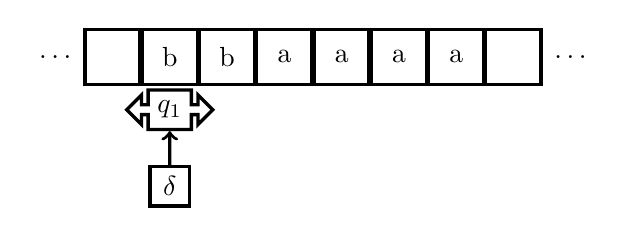
\begin{tikzpicture}
    \tikzstyle{every path}=[very thick]

    \edef\sizetape{0.7cm}
    \tikzstyle{tmtape}=[draw,minimum size=\sizetape]
    \tikzstyle{tmhead}=[arrow box,draw,minimum size=.5cm,arrow box
    arrows={east:.25cm, west:0.25cm}]
    \tikzstyle{tmprog}=[draw,minimum size=.5cm]

    %% Draw TM tape
    \begin{scope}[start chain=1 going right,node distance=-0.15mm]
        \node [on chain=1,tmtape,draw=none] {$\ldots$};
        \node [on chain=1,tmtape] {};
        \node [on chain=1,tmtape] (input) {b};
        \node [on chain=1,tmtape] {b};
        \node [on chain=1,tmtape] {a};
        \node [on chain=1,tmtape] {a};
        \node [on chain=1,tmtape] {a};
        \node [on chain=1,tmtape] {a};
        \node [on chain=1,tmtape] {};
        \node [on chain=1,tmtape,draw=none] {$\ldots$};
    \end{scope}

    %% Draw TM head below (input) tape cell
    \node [tmhead,yshift=-.3cm] at (input.south) (head) {$q_1$};
    \node [tmprog,yshift=-.7cm] at (head.south) (prog) {$\delta$};
    \draw [->] (prog) to (head);

    \end{tikzpicture}
    \nocite{tm_figure}
    \end{center}
  
\end{frame}

\begin{frame}
  \frametitle{Some results on TM}

  \begin{itemize}
    \item The \textbf{halting problem} is undecidable.
    \item The \textbf{blank tape halting problem} is undecidable.
    \begin{itemize}
      \item %TODO
    \end{itemize}
  \end{itemize}

  
\end{frame}

\begin{frame}
  \frametitle{Some Results on FOL}

  \begin{itemize}
    \item Completeness: a sentence $\phi$ is valid iff it is provable
    \item Proofs can be enumerated $\longrightarrow$ valid $\FO$ sentences
    recursively enumerable
  \end{itemize}

  \begin{definition}[Validity]
    All structures $\structa$, finite or infinite, are models of $\phi$.
    ($\structa \models \phi$)
  \end{definition}
  
\end{frame}

\section{Trakhtenbrot's Theorem}

\begin{frame}
  \frametitle{Trakthenbrot's Theorem and Failure of Completeness}

  \begin{definition}[Finite Satisfiability]
    Given a vocabulary $\sigma$, a sentence $\phi$ in that vocabulary is called
    finitely satisfiable if there is a finite structure $\structa \in
    \mathrm{STRUCT}[\sigma]$ such that $\structa \models \phi$.
  \end{definition}
  
  \pause

  \begin{theorem}[Trakhtenbrot]
    For every relational vocabulary $\sigma$ with at least one binary relation
    symbol, it is undecidable whether a sentence $\phi$ of vocabulary
    $\sigma$ is finitely satisfiable.
  \end{theorem}

\end{frame}

\begin{frame}
  \frametitle{Proof Idea}

  \begin{itemize}
    \item Code Turing machines in $\FO$
    \item For every TM $M$, construct a sentence $\phi_M$ of vocabulary $\sigma$
    such that $\phi_M$ is finitely satisfiable iff $M$ halts on the empty input.
  \end{itemize}

  
\end{frame}

\section{}
\bibliography{presentation}
\bibliographystyle{plain}

\end{document}
